% vim:ft=tex

\section{Data Prediction with MLPRegressor}\label{sec:mlp}
Since we wanted to implement the prediction algorithm in Python we used the library \emph{Scikit Learn} which provides a class \emph{\acf{mlp}} with according functions.
As we wanted to train a non-linear model we decided to use a Multi-layer Perceptron since it can learn a non-linear function approximator for either classification or regression. However  the \acs{mlp} uses backpropagation which is the most widely used algorithm for supervised learning with multi-layered feed-forward networks \cite{riedmiller1993direct}, this algorithm was implemented to train a prediction model for the rental bike usage on a daily base.\\\\
The outcome of of the Data Profiling Part 2, as described in chapter \ref{sec:mlp} served as a basis for the prediction.
As a first implementation we used the following data as an input for the feature matrix: \emph{Month, Weekday, Day, Season, Daily Weather, Daily Weather Past, Humidity, Humidity Past, Windspeed, Windspeed Past, Apparent Temperature (Avg), Apparent Temperature (Avg) Past, Rented Bikes}. Since we assume that weather conditions play an important role in bike usage we decided to add weather data. Another assumption was that on weekdays the frequency will rise, because a lot of people use rented bikes to travel to work. Furthermore we added the number of rentals of today in order to predict the ones of tomorrow. Therefore \emph{Rented Bikes Future} served as our target variable which is to predicted.\\
Since the \acs{mlp} works with data represented as dense and sparse numpy arrays of floating point values, data had to be encoded accordingly beforehand. Therefore we mapped all of the ordinal scaled data like \emph{Month, Weekday, Season, Daily Weather} to numerical data, by implementing a dictionary which assigns numerical values to ordinal data. E. g. For the weekdays we used the following dictionary:
\begin{lstlisting}[language=bash,breaklines=true]
"Weekday": {"Monday": 1, "Tuesday": 2, "Wednesday": 3, "Thursday": 4,"Friday": 5, "Saturday": 6, "Sunday":7 }
\end{lstlisting}
After the encoding we split the data into 80 \% training data and 20\% test data.
Since the \acs{mlp} is sensitive to feature scaling we normalized the data accordingly to the activation function. Since we used the \emph{logistic} activation function which expects values between [0,1] we normalized the feature matrix as well as the target variable beforehand. Scikit Learn provides several scaling mechanism to rescale the data. 
After data was scaled we applied the \acs{mlp} with \emph{logistic} as an activation function and ten hidden layers with five neurons. After the prediction we denormalized the data back to its original state. In order to rate the accuracy of the prediction we computed the \acf{rmse} which measures the difference between actual and predicted values of a model. The less the difference respectively the value, the better is the model.
To get a better impression of how the prediction worked, the results were plotted as time series.
The time series was plotted over for years, which causes the plot to be very large. In order to make it more user friendly, we implemented an interactive plot which gives the user the opportunity to zoom into specific parts or cut out some parts to look at them more closely.
\subsection{Normalization}\label{sec:normalization}
In the first attempt we used the \emph{MinMaxScaler} which rescales the data such that all vales are in the range of [0,1].
This gave us a \acs{rmse} of 122.347. To get a better impression of what that means we plotted this result which can be seen in figure \ref{fig:mlpquantile}.
\begin{figure}[H]
\hspace{-2.8cm}
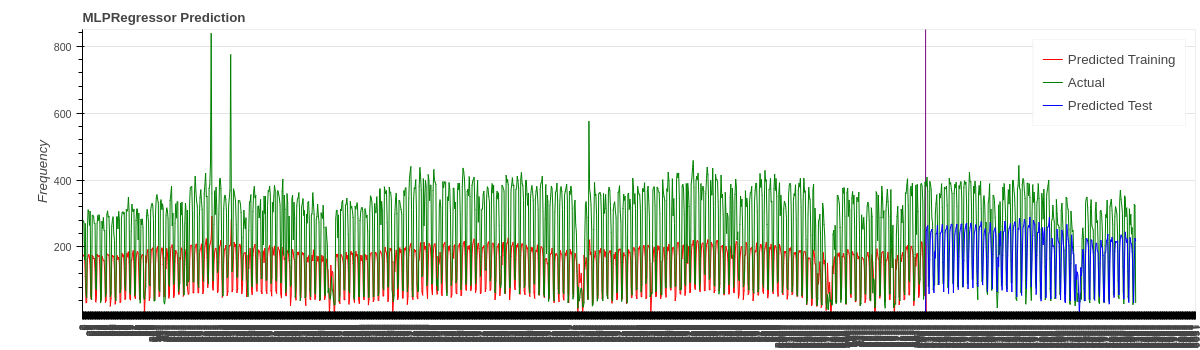
\includegraphics[width=1.4\textwidth]{img/mlpminmax}\label{fig:mlpminmax}
\captionof{figure}{Result of \acs{mlp} with MinMaxScaler}\label{fig:mlpminmax}
\end{figure}
This result shows that the prediction lack accuracy. As we found out this was caused by the MinMaxScaler, since this scaler is very sensitive to the presence of outliers. Therefore we chose another scaler for normalization which is more prone to outliers. In order to find a more suitable scaler, experiments were made with all available scalers of Scikit Learn which met the requirements for the output of the scaling. The best result was achieved by the \emph{QuantileTransformer} with a \acs{rmse} of 57.837, therefore we stuck with this normalization method.
\subsection{Feature Evaluation}\label{sec:featureeval}
In order to improve accuracy, further experiments were carried out to evaluate the features. As mentioned earlier the previous predictions were made with a feature matrix of thirteen features. To evaluate which features improve the prediction and which are useless 18 test cases were carried out. Each test case consists of different constellations of features. In the end the different \acs{rmse} values were compared, which can be seen in figure \ref{fig:evalmlp}.
\begin{figure}[H]
\hspace{-1.5cm}
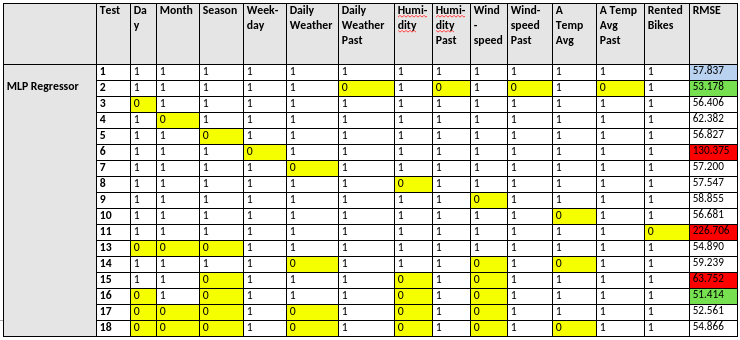
\includegraphics[width=1.2\textwidth]{img/evalmlp}\label{fig:evalmlp}
\captionof{figure}{Feature evaluation test cases}\label{fig:evalmlp}
\end{figure}
Figure \ref{fig:evalmlp} shows beneath the different test cases, included features, those are assigned to \glqq 1\grqq
 and excluded features which are assigned to \glqq 0\grqq. The first \acs{rmse} value, colored in blue depicts the prediction accuracy with all 13 features. The red colored values show the constellations which are significantly worse than the original one and in turn the green values represent the values with an increased accuracy than the original one.
\subsection{Result}\label{sec:resultmlp}
This evaluation showed that the features \emph{Weekday} and \emph{Rented Bikes} are the most important ones and in turn the features \emph{Day} and \emph{Season} are less important.
Based on our testing results we recommend to use the following nine features: \emph{Weekday, Month, Past Data, Apparent Temperature (Avg), Daily Weather} and \emph{Rented Bikes}. 
Moreover experiments with scalers showed that the \emph{QuantileTransformer} is more prone to outliers than others and is therefore the scaler of choice.\\
First plots were made with the library \emph{Matplotlib} which turns out to be very restricted and complicated to handle in order to create interactive plots. Therefore we recommend to use \emph{Bokeh} which provides easy to implement interactive plots especially for large data sets.\\
Applying the recommendations regarding scaling and feature evaluation we received a \acs{rmse} value of 51.414 which is the best value achieved during the project phase. The overall result visualized with \emph{Bokeh} can be seen in figure \ref{fig:mlpquantile}.
\begin{figure}[H]
\hspace{-2.8cm}
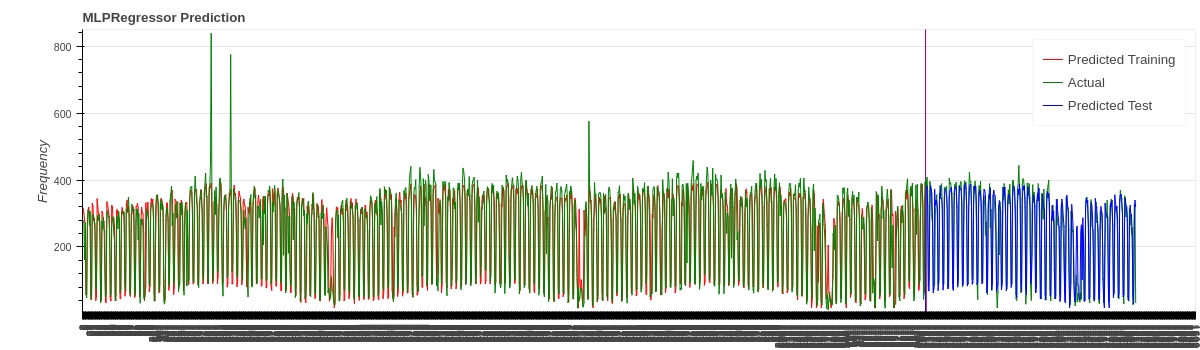
\includegraphics[width=1.4\textwidth]{img/mlpquantile}\label{fig:mlpquantile}
\captionof{figure}{Accuracy with recommended features and scaling by the QuantileTransformer}\label{fig:mlpquantile}
\end{figure}
Compared to figure \ref{fig:mlpminmax} one can see significant improvements in accuracy.\\
This model is based on the most used station, which is King´s Cross with a dataset of 1515 records. In order to confirm this model we applied it to the least used station in Farringdon Street, Holborn as well. The result can be seen in figure  \ref{fig:mlpquantile_least}.
\begin{figure}[H]
\hspace{-2.8cm}
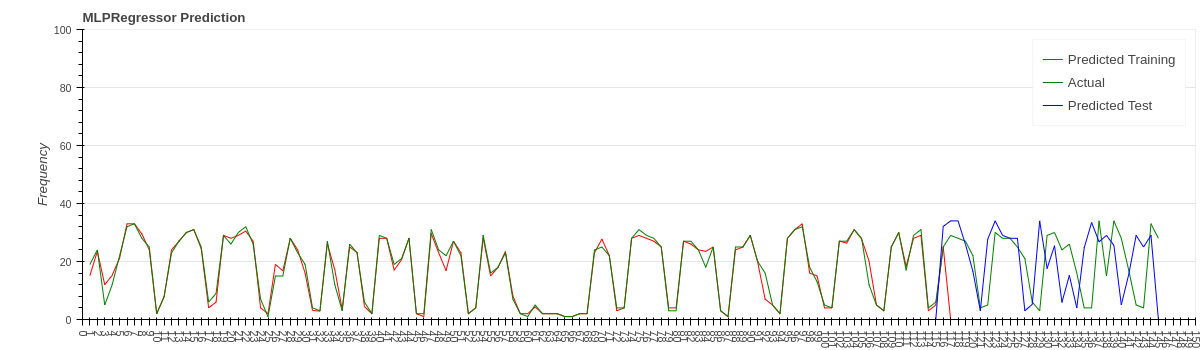
\includegraphics[width=1.4\textwidth]{img/mlpquantile_least}\label{fig:mlpquantile_least}
\captionof{figure}{Accuracy with recommended features and scaling by the QuantileTransformer}\label{fig:mlpquantile_least}
\end{figure}
The accuracy of the prediction of the least used station measures a \acs{rmse} of 9.311. This shows that the model works not only for highly frequented stations but also for stations like Farringdon Street with only 145 records.